%-----------------------------------------------
% Template para criação de resumos de projectos/dissertação
% jlopes AT fe.up.pt,   Fri Jul  3 11:08:59 2009
%-----------------------------------------------

\documentclass[9pt,a4paper]{extarticle}

%% English version: comment first, uncomment second
%\usepackage[portuguese]{babel}  % Portuguese
\usepackage[english]{babel}     % English
\usepackage{graphicx}           % images .png or .pdf w/ pdflatex OR .eps w/ latex
\usepackage{times}              % use Times type-1 fonts
\usepackage[utf8]{inputenc}     % 8 bits using UTF-8
\usepackage{url}                % URLs
\usepackage{multicol}           % twocolumn, etc
\usepackage{float}              % improve figures & tables floating
\usepackage[tableposition=top]{caption} % captions
%% English version: comment first (maybe)
\usepackage{indentfirst}        % portuguese standard for paragraphs
%\usepackage{parskip}
\usepackage{array}
\newcolumntype{M}{ >{\centering\arraybackslash} m{1cm} }
\newcolumntype{C}{ >{\centering\arraybackslash} m{2cm} }
%% page layout
\usepackage[a4paper,margin=30mm,noheadfoot]{geometry}

%% space between columns
\columnsep 12mm

%% headers & footers
\pagestyle{empty}

%% figure & table caption
\captionsetup{figurename=Fig.,tablename=Tab.,labelsep=endash,font=bf,skip=.5\baselineskip}

%% heading
\makeatletter
\renewcommand*{\@seccntformat}[1]{%
  \csname the#1\endcsname.\quad
}
\makeatother

%% avoid widows and orphans
\clubpenalty=300
\widowpenalty=300

\begin{document}

\title{\vspace*{-8mm}\textbf{\textsc{Online Advertising: Forecasting and Synthesising Web Activity Based On Historical Data}}}
\author{\emph{Pedro Manuel Santos Borges}\\[2mm]
\small{Dissertation conducted under the supervision of Prof. João Moreira, co-supervision of Prof. Hugo Ferreira}\\
\small{and company supervision of Eng. João Azevedo}\\
\small{at \emph{ShiftForward, Lda}}}
\date{}
\maketitle
%no page number 
\thispagestyle{empty}

\vspace*{-4mm}\noindent\rule{\textwidth}{0.4pt}\vspace*{4mm}

\begin{multicols}{2}

\section{Context and Framing} \label{sec:context}

The online marketing is a growing multibillion-dollar industry \cite{PricewaterhouseCoopers2013}
which is expected to continue its fast growth\cite{PricewaterhouseCoopers2013a}.

This industry is always trying to become more efficient by getting more profit from
assets it already owns. 
Web users are the major assets of this industry, which makes money by exploiting the user behavior and characteristics, in order to target them with the
perfect campaign. Each campaign has its own target parameters, which limit the target user universe.
Online marketing industry core business is centered in web users and this industry has recorded almost every footprint each user makes on the web.
Future footprints of the web users allows the measurement of the behavior of an
upcoming campaign and, with this data, it is possible to make the inventory more
profitable. Therefore, using future user data allows the adtech industry to be able to fine tune its campaigns. 
Campaigns are composed by a series of ads that share the same main idea they
want to transmit. The campaigns have a targeting typically defined as a set of
parameter definitions and rules. To be able to run the campaigns in a
simulator, their targeting can be defined as
queries over the ad requests' data. The utilization of a simulation allows to
get the results fast, test concurrent campaigns and test multiple scenarios.
The utilization of a simulation is the main reason behind
why is so important to be able to generate future ad requests' data.

The most common platforms that will benefit from this data are Custom-Built Ad
Servers and Exchanges, Sell-Side Platforms (SSPs) and
Demand-Side Platforms
(DSPs).


\section{Project} \label{sec:proj}

The online advertising market is huge and its size has been increasing in money,
campaigns and users. Both platforms that sell and buy space for ad placement
want to understand what is their value and more importantly, what will be their
value in the future. In both cases this value is mostly constrained by campaigns
and the users they want to target.

Our goal is to forecast the availability of the users in the future so we can
simulate the value of future campaigns over them.

Since we do not know which characteristics the future campaigns will have, every
detail available on the impressions needs to be forecasted, in order to
obtain the correct values when the queries are executed over the generated data.

With this said, the main goal is to be able to generate a dataset able to be used on a campaign
simulator, so we must be able to predict the values with the maximum detail
possible.

This simulator needs to have available every detail possible about every
impression in order to identify which impressions are compatible with each
campaign. The result would be expressed by number of impressions per campaign and
users target by every campaign, over time.

The approach should also only need an impression's date and user id, with all
other variables being optional.
This constraint is imposed by the multiple sources of the dataset used, since
each one of these sources could store different details and different types of
parameters about each impression, so we cannot rely on the availability of
such parameters.

The approach should be able to generate data for any source
with any parameters, based only on historical information.

To conclude, the approach's main goals are to:
\begin{itemize}
\item Correctly predict volumes of activity on an ad network for a given time in
  the future based only in past data;
\item Fill the volumes with impressions, with the maximum detail possible, to be
  able to use the obtained result on a simulator.
\end{itemize}

\section{Motivation and Goals} \label{sec:goals}

In the last few years, the online marketing has been getting more complex. In
such a way that today campaigns have a very well defined target, with
sets of rules and limitations. This poses a big problem to
simpler prediction models that normally don't predict all the parameters of the
ad request, this way limiting the parameters where queries can be done.


Nowadays, some online ads can only be imprinted if a set of very specific requirements has been fulfilled, for example,
the users had to visit an e-commerce site in the last 24 hours. This brings causality into the equation, creating a new paradigm that makes 
the more traditional methods of prediction ineffective. To solve this problem
and to be able to get fast responses to complex queries of concurrent campaigns,
simulate the algorithms executed by ad servers of the client
and ultimately parallelize the computation of the results for the
queries,
the complete future data has to be predicted. This generated data
can be used in simulations and the online campaigns can run on top of the future population.

The objective of this thesis is to develop a library capable of generating
future ad request logs using past data from the same network.
This library will have as one of its main goals the prediction of all the parameters that characterize an
ad request with the purpose of being able to query over any parameter, in other
words, the generated dataset (ad requests log) must have the same attributes as the original.

The prediction of this kind of future data is rather complex since it is
necessary to find out which users will appear in the future and which websites they
will visit and when will they do it.

\section{Approach}

\begin{figure}[H]
\centering
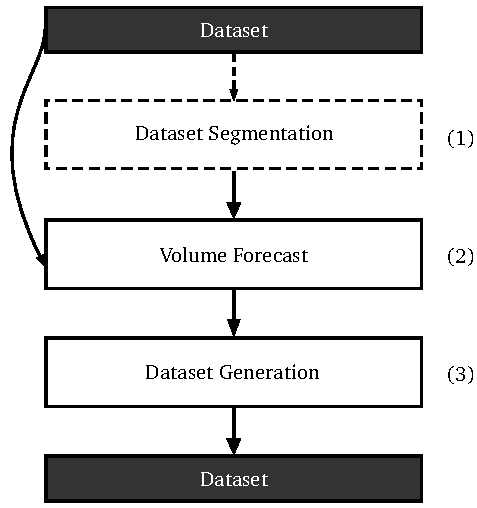
\includegraphics[width=0.3\textwidth]{high_level} \caption{ High level overview
of the approach } \label{fig:highlevel_arch} \end{figure}

As the figure~\ref{fig:highlevel_arch} makes clear, the goal of the
proposed approach is to use a dataset containing logs of the web
activity from an online advertising related network and use this information 
to generate a possible future web activity logs on the same network. 
This should be done in order to preserve tendencies and into data coherency.

This approach can be divided into three main phases:
\begin{enumerate}
\item \emph{Segmentation},
which its main purpose is divide the dataset in smaller and more predictable
datasets, in order to improve the results obtained after the second phase, mostly when there
are large quantities of data available. Datastream clustering and segmentation
by parameters are used in this phase.

\item The second phase is where the \emph{forecast of the volumes} that characterize the traffic on
  the network are done, using time series prediction methods (experiments were
  made using \emph{ARIMA}).

\item The third and last phase of the process, the more complex one, is where the volumes
generated from the phase two combined with the data provided by the original
dataset are used to \emph{generate a dataset} that represent a possible future of the
web activity on the target network.
\end{enumerate}

\section{Results}

\begin{table}[H]
\centering
\footnotesize
\begin{tabular}{m{2cm}|CMM}
  &  $\sigma$ (Real Data) & RMSE & MASE   \\ \hline
 without segmentation & 3.33      & 19.61        & 0.6760   \\ \hline
  baseline (copy past to future) & 3.33      & 19.61        & 0.6760   \\ \hline
  segmentation per parameter (browser) & 3.33      & 19.61        & 0.6760   \\ \hline
  segmentation datastream clustering (threshold 20) & 3.33      & 19.61        & 0.6760   \\ \hline
\end{tabular}

\caption[Volume
impression forecast error, safari]{Error for impression volume
forecast, using a 12h period without clustering}
\label{tab:noquery}
\end{table}

\begin{table}[H]
\centering
\footnotesize
\begin{tabular}{m{2cm}|CMM}
  &  $\sigma$ (Real Data) & RMSE & MASE   \\ \hline
 without segmentation & 3.33      & 19.61        & 0.6760   \\ \hline
  baseline (copy past to future) & 3.33      & 19.61        & 0.6760   \\ \hline
  segmentation per parameter (browser) & 3.33      & 19.61        & 0.6760   \\ \hline
  segmentation datastream clustering (threshold 20) & 3.33      & 19.61        & 0.6760   \\ \hline
\end{tabular}

\caption[Volume
impression forecast error, safari]{Error for impression volume
forecast, using a 12h period without clustering}
\label{tab:query}
\end{table}




%%English version: comment first, uncomment second
%\bibliographystyle{unsrt-pt}  % numeric, unsorted refs
\bibliographystyle{unsrt}  % numeric, unsorted refs
\bibliography{refs}

\end{multicols}

\end{document}
